% ============================================================
%  BrineWatch — Prototypes for Humanity 2026 — 2-page proposal
%  Compile with: pdflatex BrineWatch_Proposal.tex  (run twice)
% ============================================================
\documentclass[10pt,a4paper]{article}

\usepackage[margin=1.8cm,top=1.5cm,bottom=1.6cm]{geometry}
\usepackage[T1]{fontenc}
\usepackage[utf8]{inputenc}
\usepackage{lmodern}
\usepackage{microtype}
\usepackage{xcolor}
\usepackage{titlesec}
\usepackage{enumitem}
\usepackage{booktabs}
\usepackage{textcomp}
\usepackage{tikz}
\usetikzlibrary{arrows.meta,decorations.pathmorphing,positioning}
\usepackage[hidelinks]{hyperref}

% ---------- palette ----------
\definecolor{deepblue}{RGB}{11,74,124}
\definecolor{brine}{RGB}{132,59,140}
\definecolor{waterc}{RGB}{214,232,244}
\definecolor{landc}{RGB}{213,196,158}
\definecolor{accent}{RGB}{198,90,17}

% ---------- layout helpers ----------
\titleformat{\section}{\sffamily\bfseries\large\color{deepblue}}{\thesection}{0.55em}{}
\titlespacing*{\section}{0pt}{7pt plus 2pt}{3pt}
\setlist{nosep,leftmargin=1.15em}
\setlength{\parindent}{0pt}
\setlength{\parskip}{3.2pt}
\pagestyle{plain}

\newcommand{\todo}[1]{{\color{red!75!black}\textbf{[#1]}}}
\newcommand{\keyword}[1]{\textbf{\color{deepblue}#1}}

\begin{document}

% ================= TITLE BLOCK =================
\begin{minipage}[b]{0.72\textwidth}
  {\sffamily\bfseries\fontsize{23}{25}\selectfont\color{deepblue} BrineWatch}\\[3pt]
  {\sffamily\large An autonomous sentinel for the hidden cost of fresh water}\\[2pt]
  {\sffamily\small\color{black!60} Low-cost robotic mapping and live digital twins of desalination brine plumes}
\end{minipage}\hfill
\begin{minipage}[b]{0.26\textwidth}\raggedleft
  {\sffamily\small\color{black!60} Prototypes for Humanity 2026\\ Project proposal}
\end{minipage}

\vspace{3pt}
{\color{deepblue}\hrule height 1.1pt}
\vspace{4pt}

{\small\sffamily \textbf{Applicant \& team lead:} Andrea Bedei --- PhD student, University of Bologna (MSc Automotive Engineering for Intelligent Mobility, 2025) \;\textperiodcentered\; \textbf{Academic supervisors:} Giovanni Pau and Roberto Girau, University of Bologna \;\textperiodcentered\; \textbf{Industrial partner:} MBS (marine robotics)}

\vspace{2pt}
{\itshape\color{deepblue} In one sentence: a \$5{,}000 open-source underwater robot that finds, maps and watches the hypersaline plumes desalination plants discharge into the sea --- turning an invisible externality into a live, verifiable digital twin.}

% ================= 1 PROBLEM =================
\section{The problem: fresh water's invisible waste stream}
More than 300 million people drink water taken from the sea. Desalination is the lifeline of water-scarce regions --- and it is growing fast, in the Gulf and now across the Mediterranean. But every litre of fresh water leaves behind ${\approx}1.5$ litres of \keyword{brine}: hypersaline, warmer, laced with antiscalant and chlorine residues, returned to the sea through submarine outfalls at ${\approx}142$ million $\mathrm{m}^3$ \emph{per day} worldwide; four Gulf states alone produce over half of it [1], into the worst possible basin --- shallow, semi-enclosed, already the saltiest open sea on Earth.

The physics makes the harm invisible. Brine is \emph{denser} than seawater: leaving the diffuser it collapses onto the seabed and creeps downslope as a gravity current [2], forming hypersaline bottom layers that suffocate benthic life --- seagrass meadows, shellfish, the base of coastal fisheries. It also feeds a vicious cycle: a saltier intake makes every litre more energy-hungry, which produces more brine. And none of this can be seen from above: satellites and surface buoys observe the surface, while the damage happens at the bottom.

% ================= 2 GAP =================
\section{Why today's monitoring fails}
Discharge permits are granted on \keyword{CFD predictions made once, on paper}, and rarely verified against reality. In operation, compliance rests on two or three \keyword{fixed buoys} --- single points, usually at the wrong depth for a bottom-hugging plume --- and on \keyword{vessel campaigns every 3--6 months}, in which a crew lowers a probe over a grid of stations: tens of thousands of euros per survey for a few dozen point measurements, with months of darkness in between. Permits define a \keyword{mixing zone} (typically: salinity within ${\sim}5\%$ of ambient at 100--300\,m from the diffuser), yet no instrument in routine use can actually verify it in space and time. The result: regulators enforce limits they cannot measure, operators get no feedback to correct themselves, and \emph{nobody has ever seen the real 3-D shape of a plume evolving over time}.

% ================= FIGURE =================
\begin{figure}[h!]
\centering
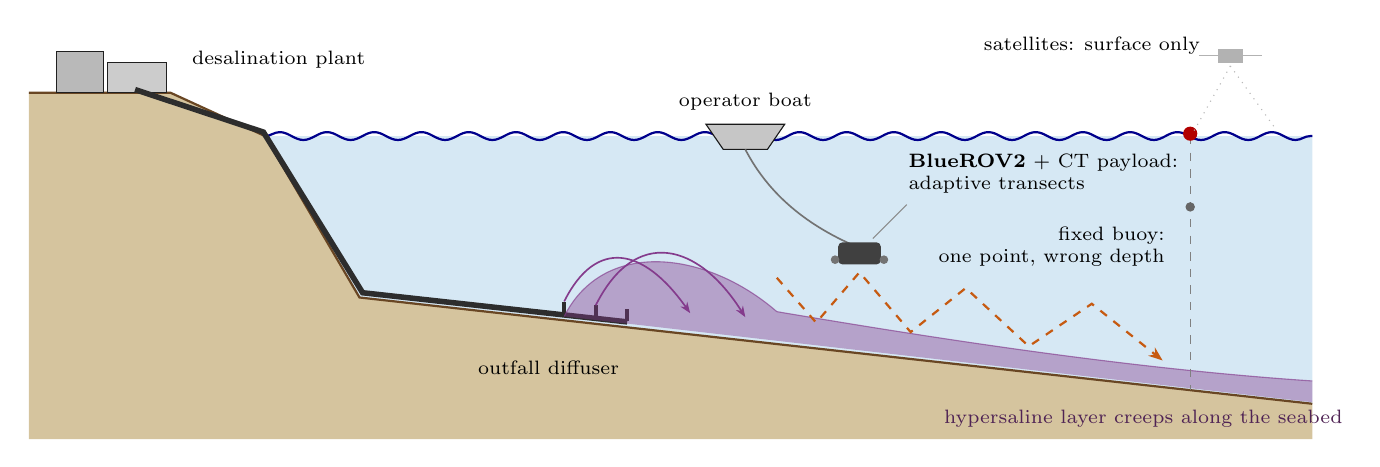
\begin{tikzpicture}[x=1cm,y=1cm,font=\scriptsize]
  % ---- water body ----
  \fill[waterc] (3.0,4.35) -- (16.3,4.35) -- (16.3,0.95) -- (4.2,2.3) -- cycle;
  % ---- land + seabed mass ----
  \fill[landc] (0,4.9) -- (1.8,4.9) -- (3.0,4.35) -- (4.2,2.3) -- (16.3,0.95) -- (16.3,0.5) -- (0,0.5) -- cycle;
  \draw[brown!55!black,thick] (0,4.9) -- (1.8,4.9) -- (3.0,4.35) -- (4.2,2.3) -- (16.3,0.95);
  % ---- sea surface ----
  \draw[blue!55!black,thick,decorate,decoration={snake,amplitude=0.05cm,segment length=0.6cm}]
      (3.0,4.35) -- (16.3,4.35);
  % ---- desalination plant ----
  \fill[gray!55] (0.35,4.9) rectangle (0.95,5.42);
  \fill[gray!40] (1.0,4.9) rectangle (1.75,5.28);
  \draw[gray!25!black] (0.35,4.9) rectangle (0.95,5.42);
  \draw[gray!25!black] (1.0,4.9) rectangle (1.75,5.28);
  \node[anchor=west,align=left] at (1.95,5.32) {desalination plant};
  % ---- outfall pipe + diffuser ----
  \draw[line width=2.0pt,gray!35!black] (1.35,4.94) -- (2.98,4.40) -- (4.24,2.36) -- (7.6,1.99);
  \foreach \x/\y in {6.8/2.085, 7.2/2.04, 7.6/1.995}{
      \draw[line width=1.4pt,gray!35!black] (\x,\y) -- (\x,\y+0.16);}
  \node[anchor=north,align=center] at (6.6,1.62) {outfall diffuser};
  % ---- brine jets ----
  \draw[-{Stealth[length=1.4mm]},brine,semithick] (6.8,2.25) .. controls (7.2,3.05) and (7.8,2.95) .. (8.4,2.1);
  \draw[-{Stealth[length=1.4mm]},brine,semithick] (7.2,2.20) .. controls (7.7,3.2) and (8.5,3.0) .. (9.1,2.05);
  % ---- plume body (gravity current) ----
  \fill[brine,fill opacity=0.40] (6.8,2.06)
      .. controls (7.3,3.05) and (8.6,2.9) .. (9.5,2.12)
      .. controls (11.4,1.8) and (13.9,1.4) .. (16.3,1.24)
      -- (16.3,0.97) -- cycle;
  \draw[brine,opacity=0.65,thin] (6.8,2.06)
      .. controls (7.3,3.05) and (8.6,2.9) .. (9.5,2.12)
      .. controls (11.4,1.8) and (13.9,1.4) .. (16.3,1.24);
  \node[align=left,anchor=west,text=brine!60!black] at (11.5,0.76)
      {hypersaline layer creeps along the seabed};
  % ---- operator boat + tether ----
  \fill[gray!45] (8.6,4.5) -- (9.6,4.5) -- (9.38,4.18) -- (8.82,4.18) -- cycle;
  \draw[gray!20!black] (8.6,4.5) -- (9.6,4.5) -- (9.38,4.18) -- (8.82,4.18) -- cycle;
  \node[anchor=south] at (9.1,4.55) {operator boat};
  \draw[black!55,semithick] (9.1,4.18) .. controls (9.4,3.6) and (9.9,3.2) .. (10.55,2.93);
  % ---- ROV ----
  \fill[rounded corners=1.5pt,black!75] (10.28,2.72) rectangle (10.82,3.0);
  \fill[black!55] (10.24,2.78) circle (0.055);
  \fill[black!55] (10.86,2.78) circle (0.055);
  \node[anchor=south west,align=left] at (11.05,3.5)
      {\textbf{BlueROV2} + CT payload:\\adaptive transects};
  \draw[black!45,thin] (11.15,3.48) -- (10.72,3.05);
  % ---- adaptive trajectory ----
  \draw[dashed,accent,thick,-{Stealth[length=1.8mm]}]
      (9.5,2.55) -- (10.0,1.98) -- (10.55,2.62) -- (11.2,1.86) -- (11.9,2.42)
      -- (12.7,1.68) -- (13.5,2.22) -- (14.4,1.5);
  % ---- fixed buoy ----
  \draw[dashed,black!50] (14.75,4.35) -- (14.75,1.12);
  \fill[red!70!black] (14.75,4.38) circle (0.09);
  \fill[black!60] (14.75,3.45) circle (0.06);
  \node[anchor=east,align=right] at (14.55,2.95) {fixed buoy:\\one point, wrong depth};
  % ---- satellite ----
  \fill[gray!60] (15.1,5.28) rectangle (15.42,5.46);
  \draw[gray!60] (14.86,5.37) -- (15.1,5.37)   (15.42,5.37) -- (15.66,5.37);
  \draw[dotted,gray!55] (15.26,5.24) -- (14.8,4.42)  (15.26,5.24) -- (15.85,4.42);
  \node[anchor=east] at (15.0,5.5) {satellites: surface only};
\end{tikzpicture}

\vspace{4pt}
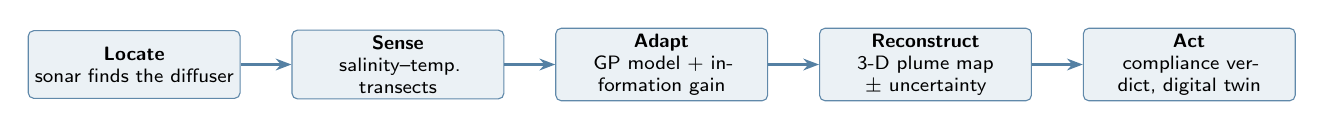
\begin{tikzpicture}[font=\scriptsize\sffamily,
    box/.style={draw=deepblue!65,fill=deepblue!8,rounded corners=2pt,align=center,
                minimum height=0.86cm,text width=2.55cm,inner sep=2pt},
    arr/.style={-{Stealth[length=2mm]},deepblue!70,thick}]
  \node[box] (a) at (0,0)    {\textbf{Locate}\\sonar finds the diffuser};
  \node[box] (b) at (3.35,0) {\textbf{Sense}\\salinity--temp.\ transects};
  \node[box] (c) at (6.7,0)  {\textbf{Adapt}\\GP model + information gain};
  \node[box] (d) at (10.05,0){\textbf{Reconstruct}\\3-D plume map $\pm$ uncertainty};
  \node[box] (e) at (13.4,0) {\textbf{Act}\\compliance verdict, digital twin};
  \draw[arr] (a) -- (b); \draw[arr] (b) -- (c); \draw[arr] (c) -- (d); \draw[arr] (d) -- (e);
\end{tikzpicture}
\caption{\small \textbf{The BrineWatch mission.} Dense brine sinks and creeps along the seabed, where satellites and fixed buoys cannot see it. A \$5k open-source ROV crosses the plume boundary with adaptive transects and turns every mission into an updated 3-D map, a compliance verdict and a living digital twin of the discharge zone.}
\label{fig:concept}
\end{figure}

% ================= 3 APPROACH =================
\section{Our approach: a robot that follows the salt}
BrineWatch turns a \$5k-class open-source ROV --- a \keyword{BlueROV2 Heavy} with low-light HD camera, Cerulean Omniscan 450 FS forward-looking imaging sonar and IMU --- plus a ${\approx}$\texteuro300 \keyword{conductivity--temperature payload} (I\textsuperscript{2}C on BlueOS) into an autonomous compliance instrument (Fig.~\ref{fig:concept}):
\begin{enumerate}
  \item \keyword{Locate} --- the sonar finds the outfall pipe and diffuser on the seabed, anchoring the survey frame.
  \item \keyword{Sense} --- continuous salinity--temperature--depth sampling along baseline transects.
  \item \keyword{Adapt} --- an online Gaussian-Process field model picks the next waypoints by expected information gain [3]: the robot concentrates effort where it matters --- the plume boundary --- \emph{following the salt} instead of mowing a blind grid.
  \item \keyword{Reconstruct} --- the posterior becomes a 3-D isohaline map with explicit uncertainty.
  \item \keyword{Act} --- the map is checked automatically against permit thresholds; every mission updates a \keyword{living digital twin} of the discharge zone: trends, seasonal drift, alerts, and a feedback loop the plant can use to modulate dilution or discharge timing.
\end{enumerate}
The planner is vehicle-agnostic (waypoint interface, MAVLink-ready): it ports to any ROV/AUV, and tomorrow to residency stations for fully unattended operation.

% ================= 4 ADVANTAGES =================
\section{Measurable advantages}
\begin{center}\small
\begin{tabular}{@{}p{3.0cm}p{6.0cm}p{7.0cm}@{}}
\toprule
 & \textbf{Today (vessel + buoys)} & \textbf{BrineWatch} \\
\midrule
Cost per survey   & \texteuro20--50k (vessel, crew, winch) & ${\approx}$\texteuro500 all-in per mission \\
Frequency         & every 3--6 months & weekly or on demand \\
Data              & a few dozen point casts & thousands of samples; full 3-D field $+$ uncertainty \\
Output            & static report, months later & same-day compliance verdict; live digital twin \\
Barrier to entry  & survey vessel and specialist crew & \$5k open-source ROV --- any municipality or lab \\
\bottomrule
\end{tabular}
\end{center}
Adaptive sampling is itself a quantified gain: informative path planning reports 2--3$\times$ efficiency over fixed grids in field monitoring [3]; our simulation study benchmarks exactly this for benthic brine plumes --- same battery, lawnmower vs.\ adaptive --- and reports reconstruction error side by side.

% ================= 5 VALIDATION =================
\section{Validation plan: honest and time-boxed}
\textbf{Phase 1 --- by submission (simulation-complete).} Full-mission demonstration in \keyword{HoloOcean 2.x} [4] (Unreal Engine 5.3): official BlueROV2 Heavy model, simulated forward-looking imaging sonar and configurable currents. The plume is an analytic negatively-buoyant jet + seabed gravity current (Roberts-type parameterization [2]) advected by an idealized tide; a virtual CT sensor samples the field at the vehicle pose with realistic noise. Deliverables: mission video, lawnmower-vs-adaptive benchmark at equal battery, dashboard with automatic compliance verdict. We deliberately declare the analytic plume: in deployment, BrineWatch is precisely the instrument that \emph{validates CFD models against reality}.

\textbf{Phase 2 --- with award support.} Integration of the CT payload on our physical BlueROV2 (${\approx}$\texteuro300 sensor), tank and harbour trials, then a pilot survey at a partner desalination outfall with a utility or environmental regulator --- the natural hosts are in the Gulf itself.

% ================= 6 IMPACT =================
\section{Real-world impact}
\keyword{Water security.} Desalination capacity will keep growing with climate stress --- and brine with it. Making discharge verifiable builds the social licence for the technology hundreds of millions of people drink from; the intake-salinity feedback also protects plant efficiency.
\keyword{Ecosystems and livelihoods.} Continuous bottom-layer monitoring protects seagrass and benthic habitats --- and the artisanal fisheries above them.
\keyword{Democratized enforcement.} At two orders of magnitude below vessel-survey cost, any coastal city, regulator or university lab can hold an outfall accountable --- in the Gulf, the Mediterranean, or anywhere the sea is asked to pay for fresh water.
\keyword{Beyond brine.} The same platform audits sewage outfalls, desalination intakes and port infrastructure: one sentinel for the submerged interface between cities and the sea. \emph{(SDG 6 \textperiodcentered\ 14 \textperiodcentered\ 9)}

\vspace{2pt}
{\color{deepblue}\hrule height 0.7pt}
\vspace{3pt}
{\footnotesize
[1] E.~Jones \emph{et al.}, ``The state of desalination and brine production: a global outlook,'' \emph{Sci.\ Total Environ.}\ 657, 2019.\;
[2] P.\,J.\,W.~Roberts, ``Near-field flow dynamics of concentrate discharges and diffuser design,'' in \emph{Intakes and Outfalls for Seawater RO Desalination}, Springer, 2015.\;
[3] G.~Hitz \emph{et al.}, ``Adaptive continuous-space informative path planning for online environmental monitoring,'' \emph{J.\ Field Robotics} 34(8), 2017.\;
[4] E.~Potokar \emph{et al.}, ``HoloOcean: an underwater robotics simulator,'' \emph{IEEE ICRA}, 2022; ``A preview of HoloOcean 2.0,'' arXiv:2510.06160, 2025.
}

\end{document}
